\begin{figure}[h!]
    \centering
    \caption{Relationship between log rents and the minimum wage measures, 
             sample of affected ZIP code-months}
    \label{fig:rents_mw_non_parametric}
    
    \begin{minipage}{.95\textwidth} \centering
        (a) Raw data
        \vspace{1mm}
    \end{minipage}
    \begin{subfigure}{0.49\textwidth}
        \caption*{Residence MW}
        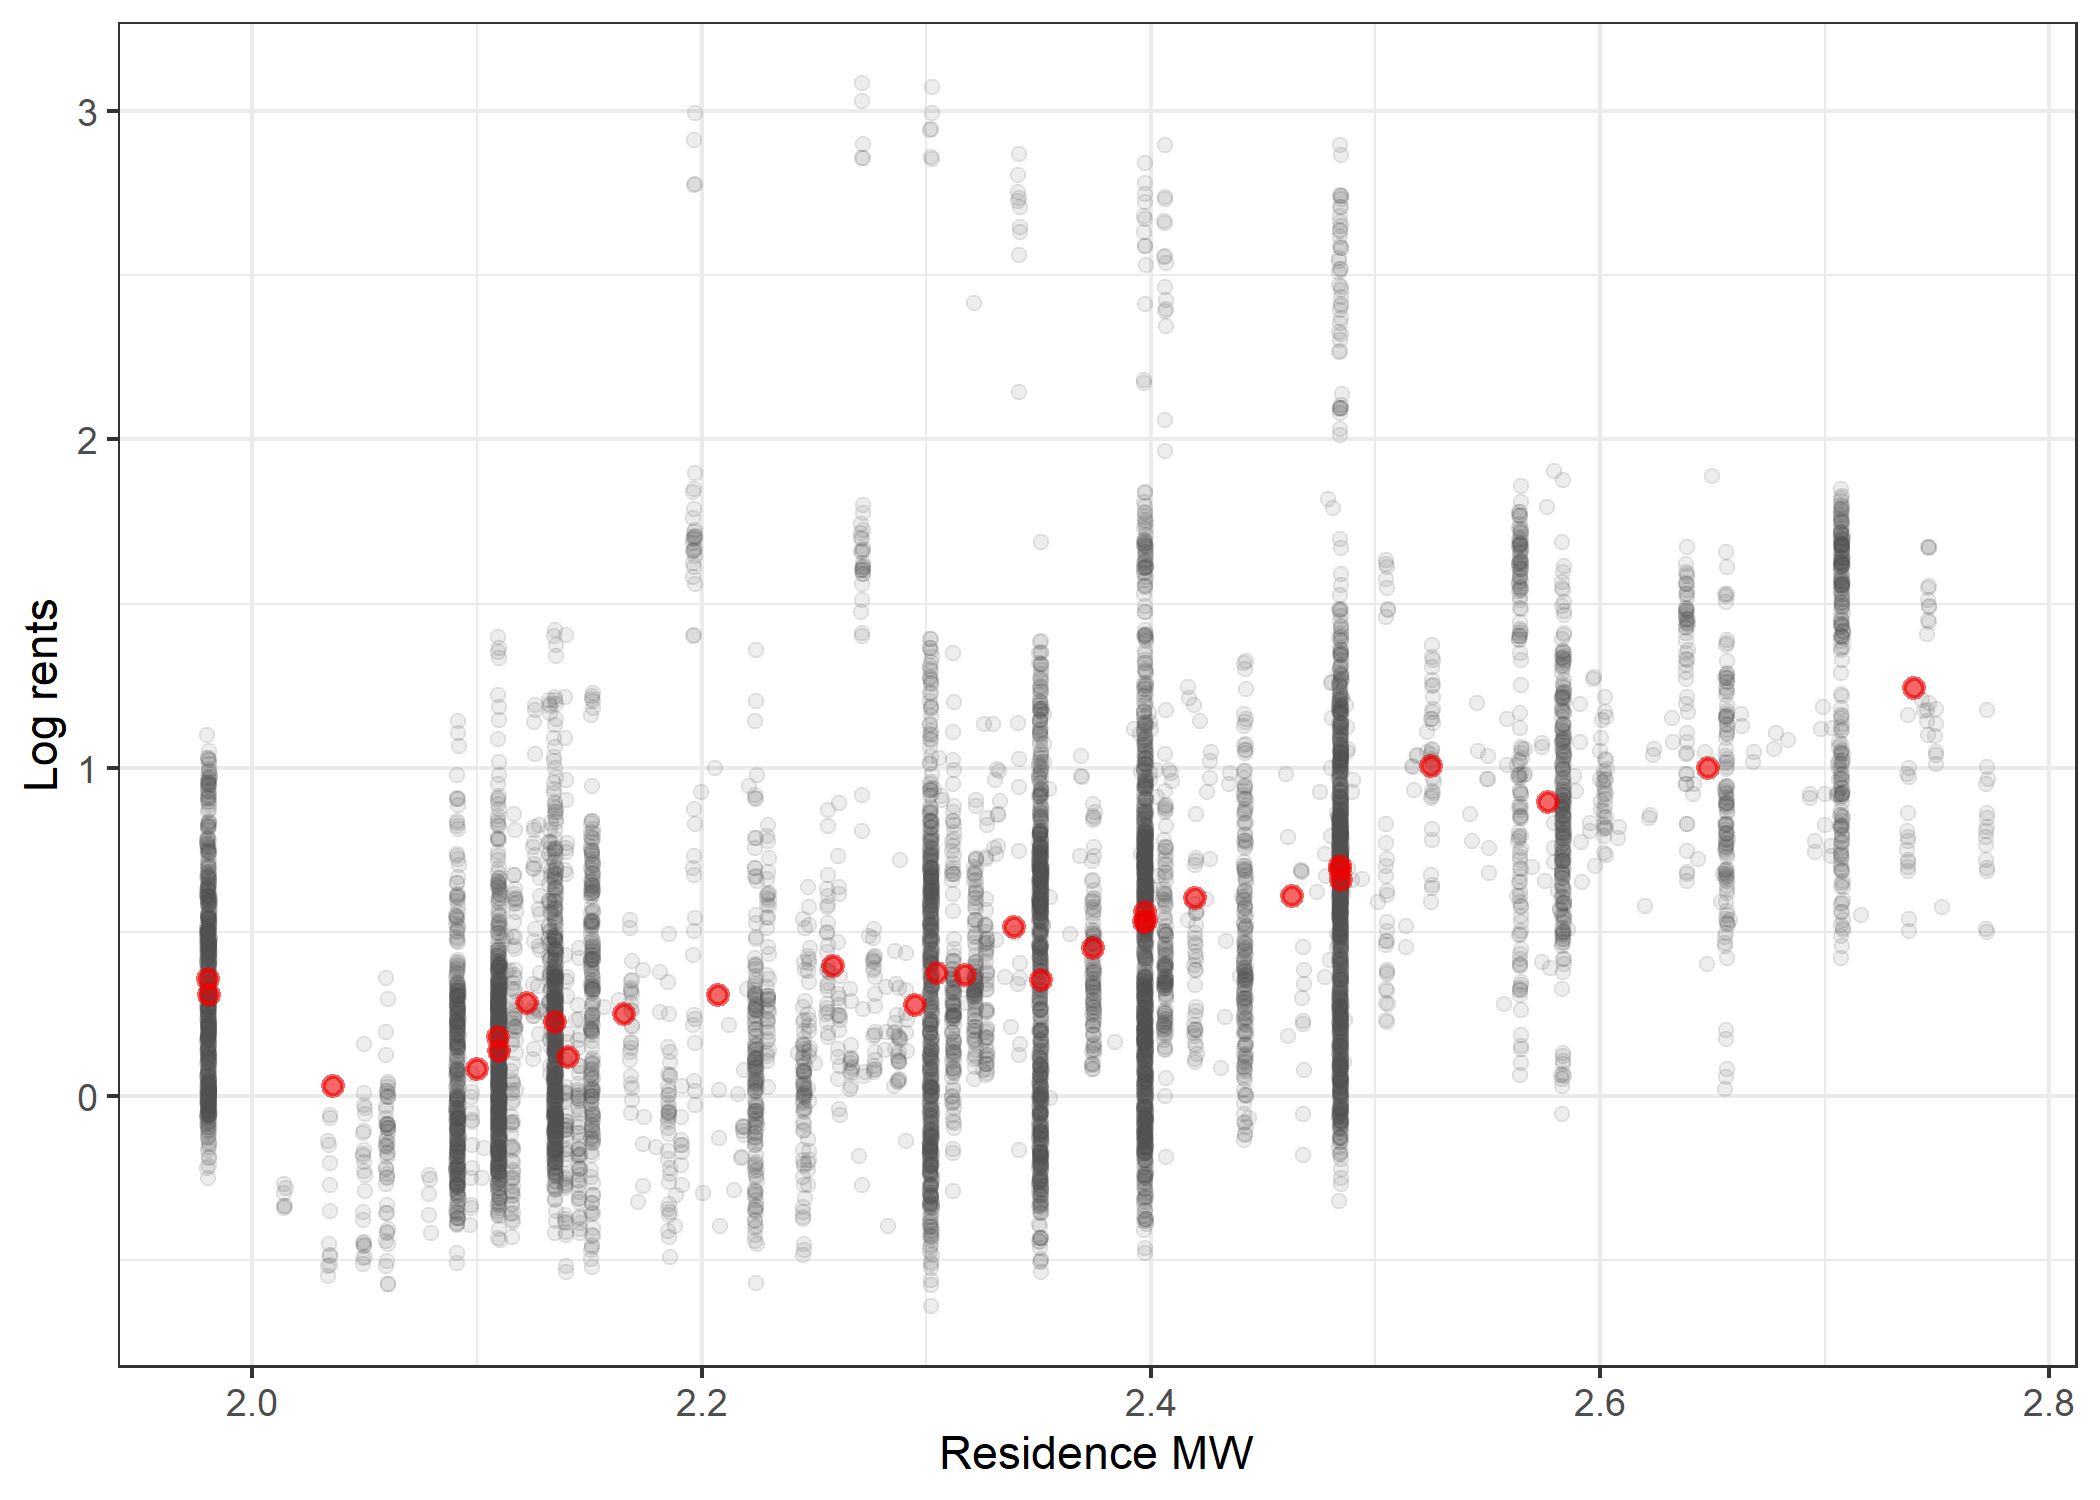
\includegraphics[width = 1\textwidth]{non_parametric/output/cbsa_month_mw_res.png}
    \end{subfigure}%
    \begin{subfigure}{0.49\textwidth}
        \caption*{Workplace MW}
        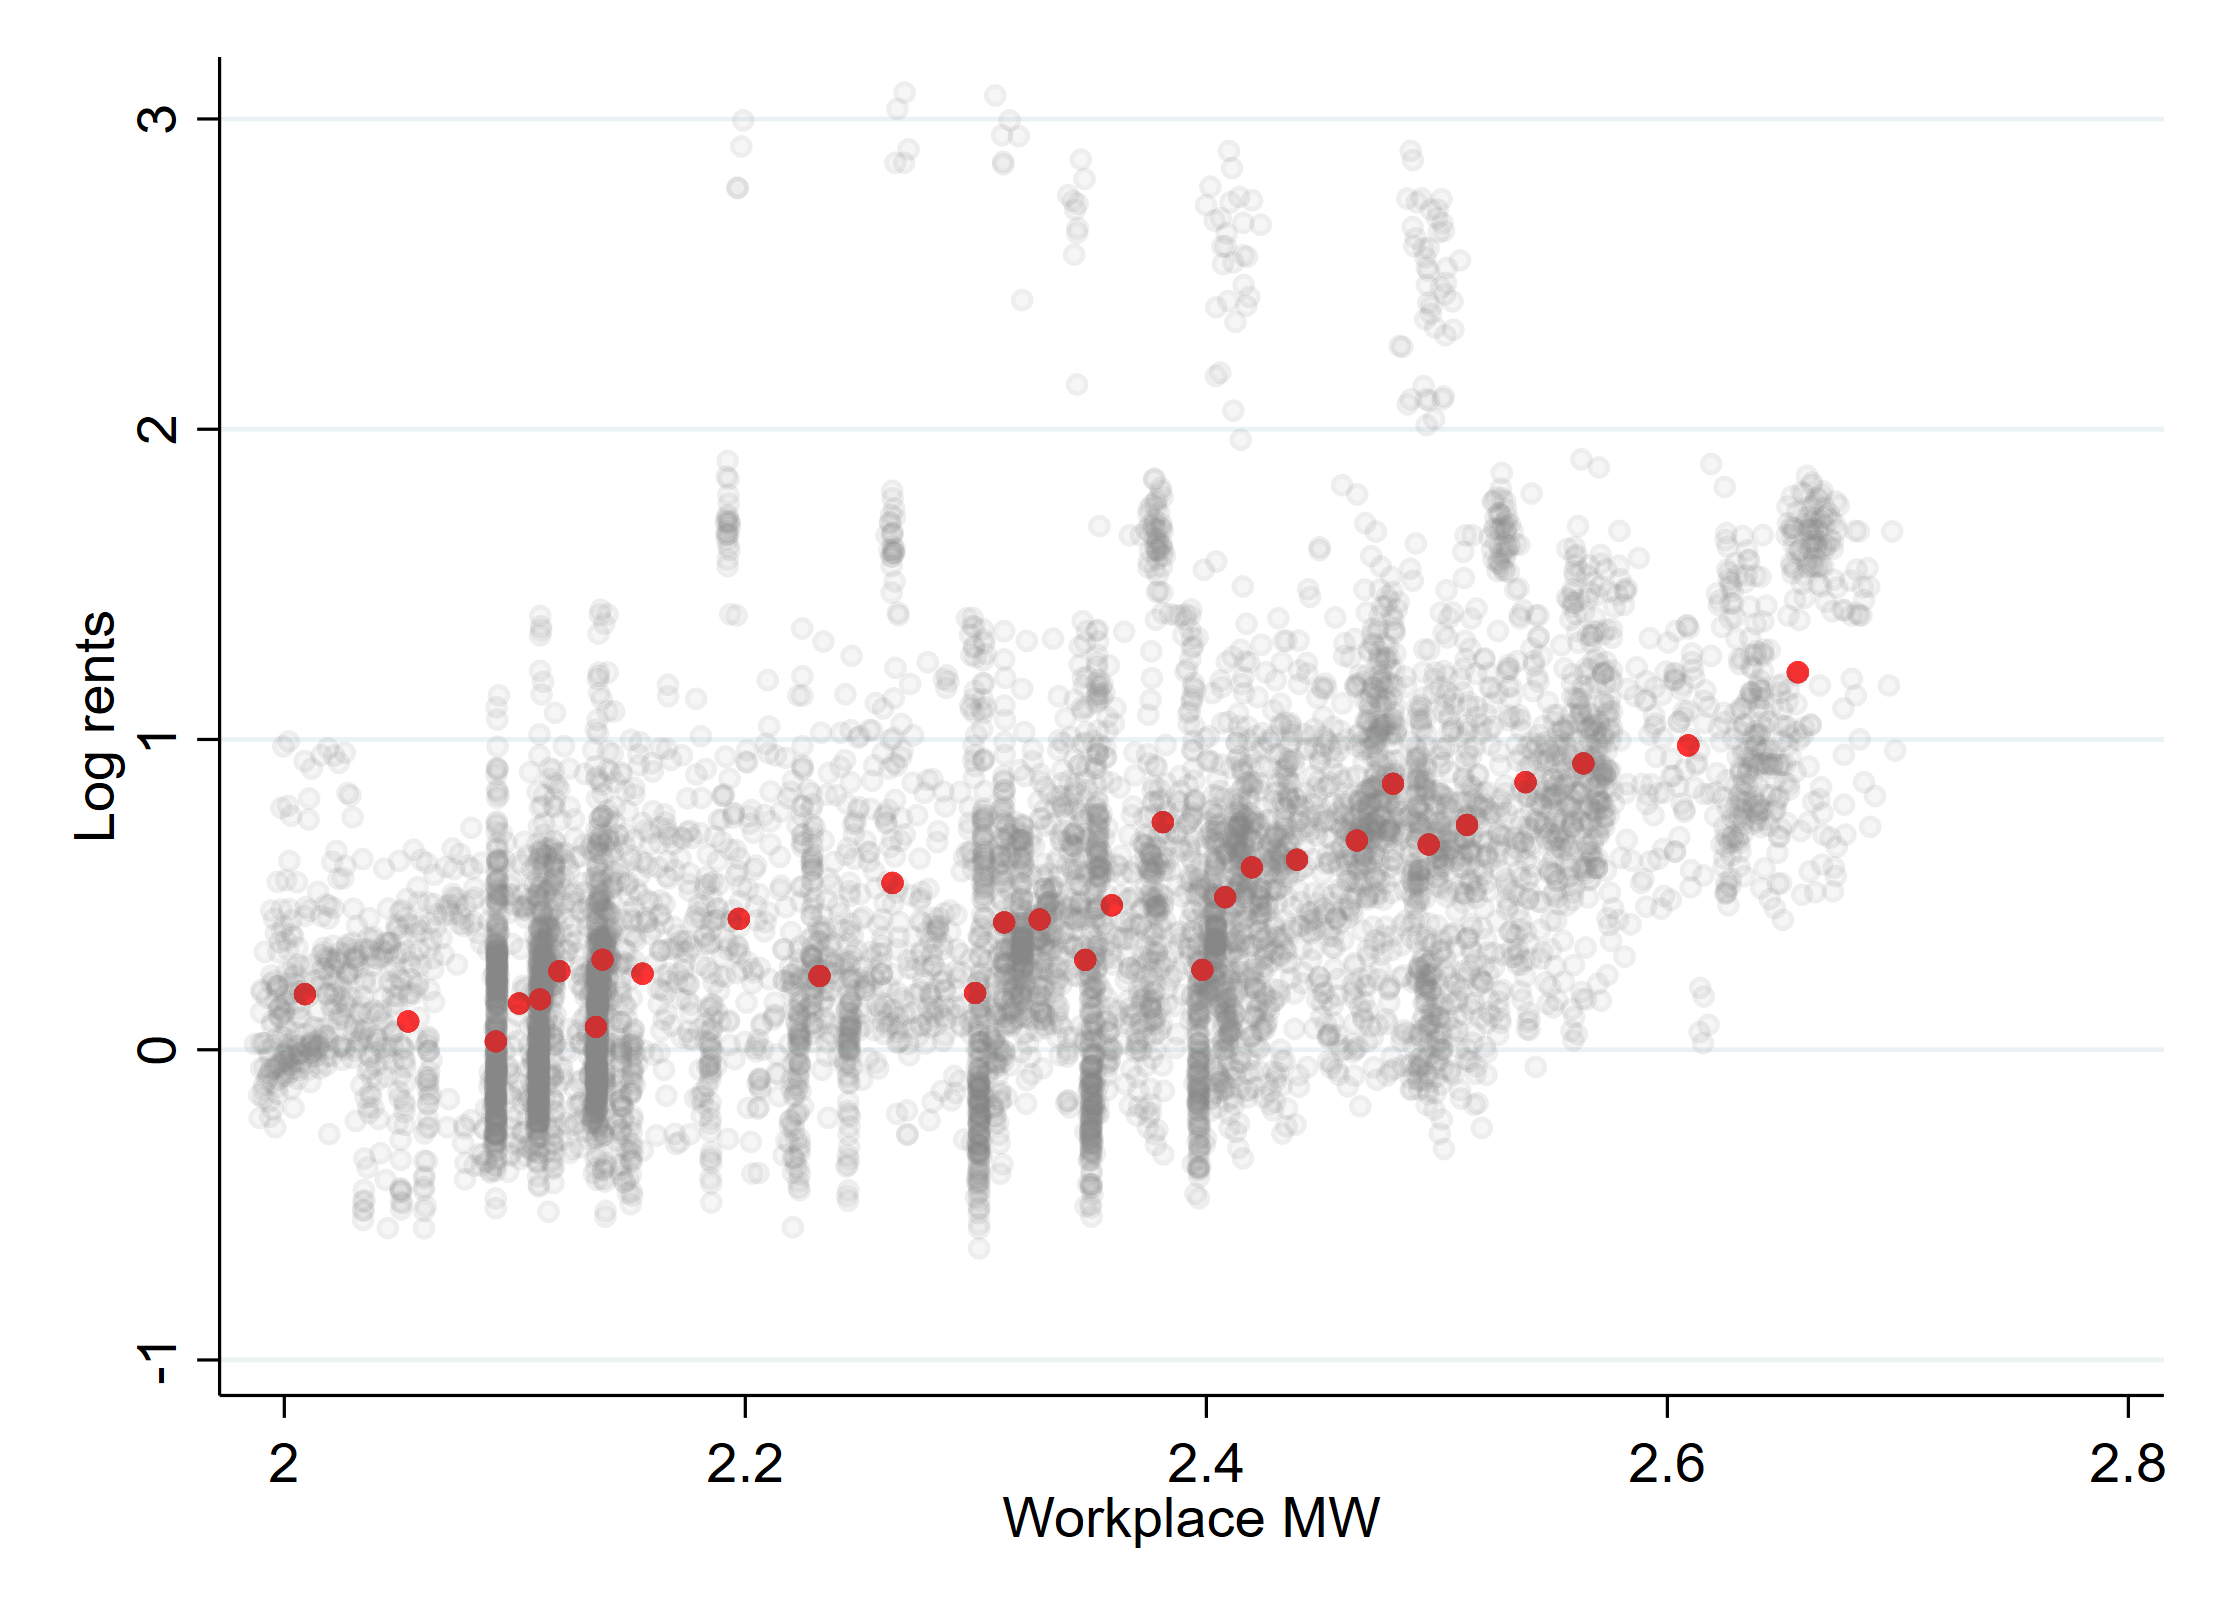
\includegraphics[width = 1\textwidth]{non_parametric/output/cbsa_month_mw_wkp.png}
    \end{subfigure}\\

    \vspace{2mm}
    \begin{minipage}{.95\textwidth} \centering
        (b) Conditional on ZIP code FE and the other MW measure
        \vspace{1mm}
    \end{minipage}
    \begin{subfigure}{0.49\textwidth}
        \caption*{Residence MW}
        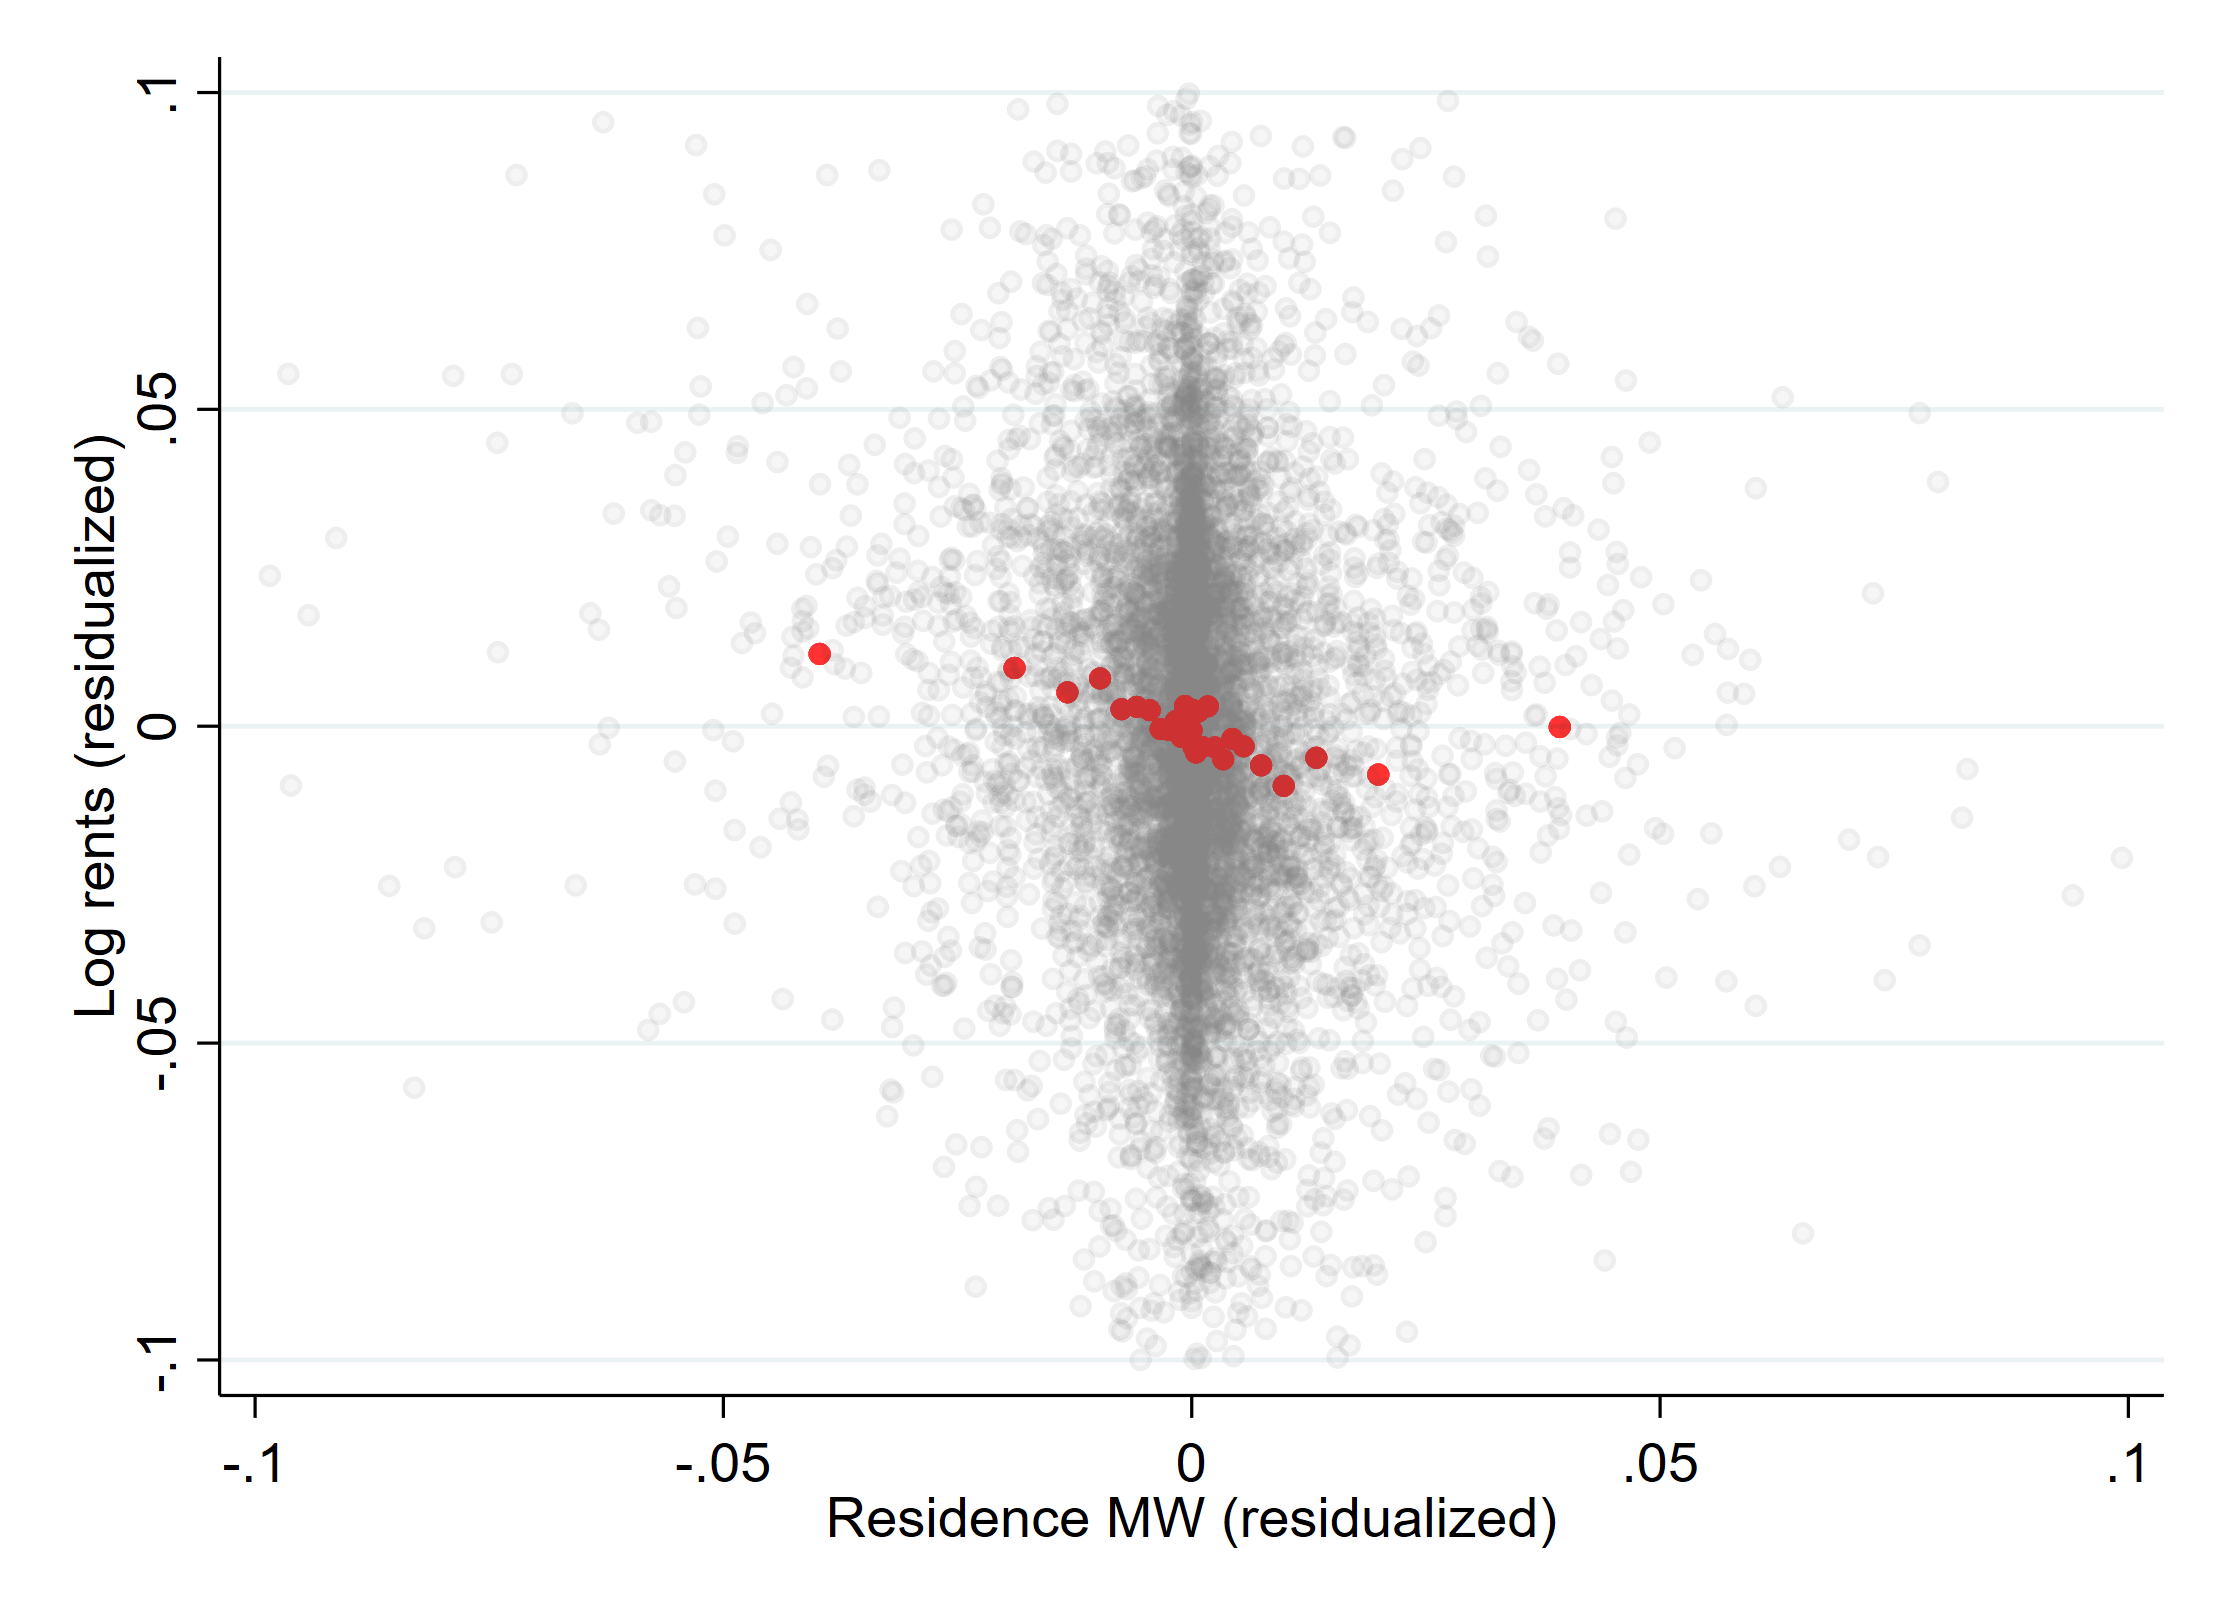
\includegraphics[width = 1\textwidth]{non_parametric/output/cbsa_month_mw_res_resid_mw_wkp_dec.png}
    \end{subfigure}%
    \begin{subfigure}{0.49\textwidth}
        \caption*{Workplace MW}
        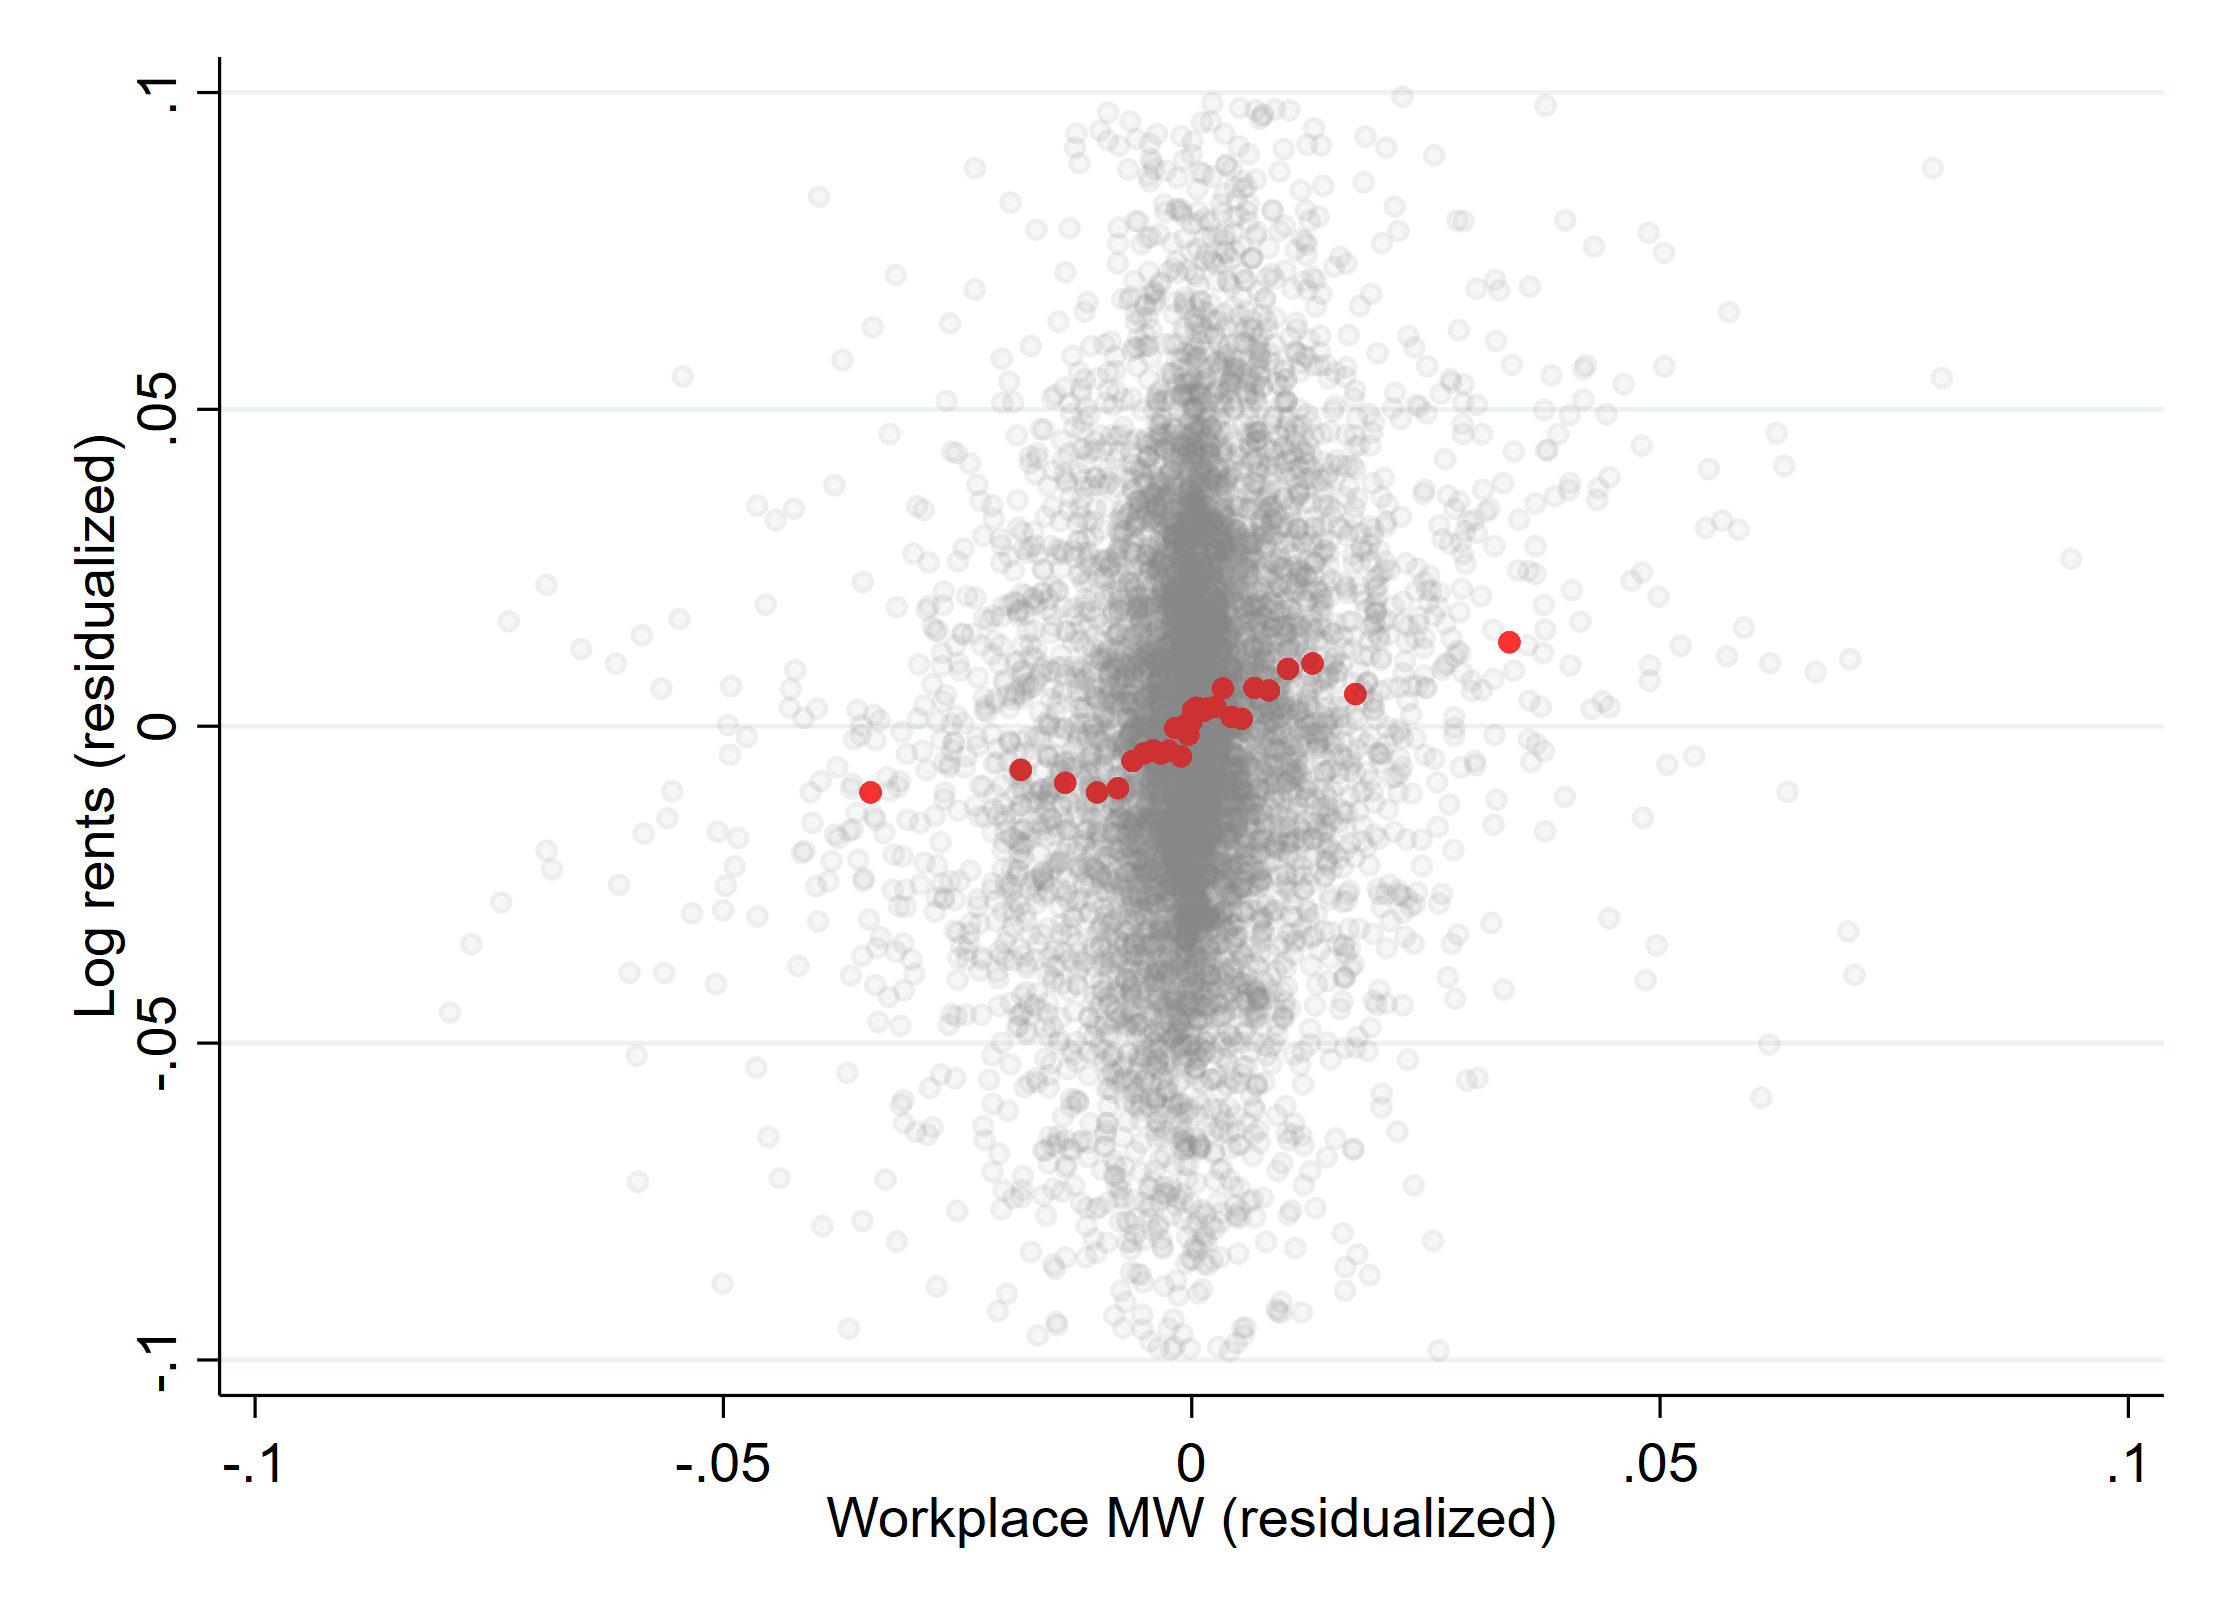
\includegraphics[width = 1\textwidth]{non_parametric/output/cbsa_month_mw_wkp_resid_mw_res_dec.png}
    \end{subfigure}

    \begin{minipage}{.95\textwidth} \footnotesize
        \vspace{3mm}
        Notes:
        Data are from Zillow and LODES.
        We keep in the sample ZIP code-month observations located in CBSAs where 
        there was some statutory MW increase in the month of interest. 
        The rents variable correspond to log rents per square foot in the SFCC 
        category.
        The workplace MW measure uses LODES data from the closest prior year.
        Panel (a) shows the raw relationship between log rents and workplace 
        and residence MW levels.
        Panel (b) shows the same relationship using residuals from regressions 
        on ZIP code and 100 indicators of the other MW measure.
        Red dots correspond to 30 equally-sized bins of the $x$-axis variable.
    \end{minipage}
\end{figure}